\documentclass{ltjsarticle}
\usepackage{luatexja}
%Packages -----------------------
\usepackage{adjustbox}
\usepackage{listings}
\usepackage[euler]{textgreek}
\usepackage{enumitem}
\usepackage[margin=30mm]{geometry}
\usepackage{comment}
\usepackage{hyperref}
\usepackage{float}
\usepackage{textcomp}
\usepackage{xparse}
%Circuit ------------------------
%Command ---–--------------------
\renewcommand{\figurename}{図}
\renewcommand{\baselinestretch}{1.1}
\lstset{
    numbers=left,
    basicstyle={\ttfamily},
    identifierstyle={\small},
    commentstyle={\smallitshape},
    keywordstyle={\small\bfseries},
    ndkeywordstyle={\small},
    stringstyle={\small\ttfamily},
    frame={tb},
    breaklines=true,
    columns=[l]{fullflexible},
    xrightmargin=0\zw,
    xleftmargin=3\zw,
    numberstyle={\scriptsize},
    stepnumber=1,
    %numbersep=1,
    lineskip=-0.5ex,
    keywordstyle=\color[HTML]{e10021},
    commentstyle=\color{gray},
    emph=CascadeObjectDetector,
    emphstyle=\color{blue}
}
\usepackage[compatibility,siunitx,  americanvoltages, americancurrents, europeanresistors, europeaninductors, americanports,%
  straightlabels, fetbodydiode, straightvoltages]{circuitikz}
\usepackage{tikz,amsmath, amssymb,bm,color,pgfkeys,siunitx,ifthen,ulem}
\usepackage{pgfplots}
\pgfplotsset{compat=1.14}
\usetikzlibrary{shapes,arrows}
%\usepackage{agaramondc}					% Adobe Garamond, custom shape
%\renewcommand{\shapedefault}{rtl} % rtl: roman tabular lining

\makeatletter

%% bandstop filter (adapted from highpass)
\pgfcircdeclarebipole{}{\ctikzvalof{bipoles/highpass/width}}{*bandstop}{\ctikzvalof{bipoles/highpass/width}}{\ctikzvalof{bipoles/highpass/width}}{
	\pgf@circ@res@step = \ctikzvalof{bipoles/highpass/width}\pgf@circ@Rlen
	\divide \pgf@circ@res@step by 2
	
	\pgfpathmoveto{\pgfpoint{\pgf@circ@res@left}{\pgf@circ@res@zero}}
	\pgf@circ@res@other = \pgf@circ@res@left
	\advance\pgf@circ@res@other by \pgf@circ@res@step 
	
	\ifpgf@circuit@dashed
	\pgfsetdash{{0.1cm}{0.1cm}}{0cm} 
	\fi	
	
	% draw outer box
	\pgfsetlinewidth{\pgfkeysvalueof{/tikz/circuitikz/bipoles/thickness}\pgfstartlinewidth}
	\pgfpathrectanglecorners{\pgfpoint{\pgf@circ@res@left}{\pgf@circ@res@up}}{\pgfpoint{\pgf@circ@res@right}{\pgf@circ@res@down}}
	\pgfusepath{draw}
	
	\ifpgf@circuit@inputarrow
	{
		\advance \pgf@circ@res@left by -.5\pgfkeysvalueof{/tikz/circuitikz/bipoles/thickness}\pgfstartlinewidth
		\pgftransformshift{\pgfpoint{\pgf@circ@res@left}{0pt}}
		\pgfnode{inputarrow}{tip}{}{pgf@inputarrow}{\pgfusepath{fill}}
	}
	\fi
	
	% rotate inner symbol
	\def\pgfcircmathresult{\expandafter\pgf@circ@stripdecimals\pgf@circ@direction\pgf@nil}
	\ifnum \pgfcircmathresult > 45 \ifnum \pgfcircmathresult < 135
	\pgftransformrotate{270}
	\fi\fi
	\ifnum \pgfcircmathresult > 134 \ifnum \pgfcircmathresult < 225  % 134 degree, because >= 135 is not possible
	\pgftransformrotate{180}
	\fi\fi
	\ifnum \pgfcircmathresult > 224 \ifnum \pgfcircmathresult < 315
	\pgftransformrotate{90}
	\fi\fi
	
	% draw inner symbol
	\pgfsetdash{}{0pt}	% always draw solid line for inner symbol
	\pgfsetarrows{-} %never draw arrows
	\pgfsetlinewidth{\pgfstartlinewidth}
	\pgfpathmoveto{\pgfpoint{-0.5\pgf@circ@res@step}{0.5\pgf@circ@res@step}}
	\pgfpathsine{\pgfpoint{.25\pgf@circ@res@step}{.25\pgf@circ@res@step}}
	\pgfpathcosine{\pgfpoint{.25\pgf@circ@res@step}{-.25\pgf@circ@res@step}}
	\pgfpathsine{\pgfpoint{.25\pgf@circ@res@step}{-.25\pgf@circ@res@step}}
	\pgfpathcosine{\pgfpoint{.25\pgf@circ@res@step}{.25\pgf@circ@res@step}}
	\pgfusepath{draw}
	
	\pgfpathmoveto{\pgfpoint{-0.5\pgf@circ@res@step}{0}}
	\pgfpathsine{\pgfpoint{.25\pgf@circ@res@step}{.25\pgf@circ@res@step}}
	\pgfpathcosine{\pgfpoint{.25\pgf@circ@res@step}{-.25\pgf@circ@res@step}}
	\pgfpathsine{\pgfpoint{.25\pgf@circ@res@step}{-.25\pgf@circ@res@step}}
	\pgfpathcosine{\pgfpoint{.25\pgf@circ@res@step}{.25\pgf@circ@res@step}}
	\pgfusepath{draw}
	\pgfpathmoveto{\pgfpoint{-0.15\pgf@circ@res@step}{-0.15\pgf@circ@res@step}}
	\pgfpathlineto{\pgfpoint{0.15\pgf@circ@res@step}{0.15\pgf@circ@res@step}}
	\pgfusepath{draw}
	
	\pgfpathmoveto{\pgfpoint{-0.5\pgf@circ@res@step}{-0.5\pgf@circ@res@step}}
	\pgfpathsine{\pgfpoint{.25\pgf@circ@res@step}{.25\pgf@circ@res@step}}
	\pgfpathcosine{\pgfpoint{.25\pgf@circ@res@step}{-.25\pgf@circ@res@step}}
	\pgfpathsine{\pgfpoint{.25\pgf@circ@res@step}{-.25\pgf@circ@res@step}}
	\pgfpathcosine{\pgfpoint{.25\pgf@circ@res@step}{.25\pgf@circ@res@step}}
	\pgfusepath{draw}
	%	\pgfpathmoveto{\pgfpoint{-0.15\pgf@circ@res@step}{-0.65\pgf@circ@res@step}}
	%	\pgfpathlineto{\pgfpoint{0.15\pgf@circ@res@step}{-0.35\pgf@circ@res@step}}
	%	\pgfusepath{draw}
}

\tikzset{
	*bandstop/.style={\circuitikzbasekey, /tikz/to path=\pgf@circ@*bandstop@path},
}
\def\pgf@circ@*bandstop@path#1{\pgf@circ@bipole@path{*bandstop}{#1}}




\makeatother

\usetikzlibrary{backgrounds,calc,positioning}

\usetikzlibrary{circuits.ee.IEC}
\usetikzlibrary{arrows}


% sym32a style

\ctikzset{tripoles/mos style/arrows}
\ctikzset{
	/tikz/circuitikz/quadpoles/coupler/width=1,%1.3
	/tikz/circuitikz/quadpoles/coupler/height=0.952,%1.3
	/tikz/circuitikz/quadpoles/coupler2/width=1,%1.3
	/tikz/circuitikz/quadpoles/coupler2/height=0.952,%1.3
	/tikz/circuitikz/quadpoles/transformer/width=1.425,%1.5
	/tikz/circuitikz/quadpoles/transformer/height=1.425,%1.5
	/tikz/circuitikz/quadpoles/transformer core/width=1.425,%1.5
	/tikz/circuitikz/quadpoles/transformer core/height=1.425,%1.5
	/tikz/circuitikz/quadpoles/gyrator/width=1.425,%1.5
	/tikz/circuitikz/quadpoles/gyrator/height=1.425,%1.5
	%/tikz/circuitikz/monopoles/tlinestub/width=0.1875,%0.25 no effect!
	/tikz/circuitikz/tripoles/american and port/height=0.95,%.8
	/tikz/circuitikz/tripoles/american nand port/height=0.95,%.8
	/tikz/circuitikz/tripoles/american or port/height=0.95,%.8
	/tikz/circuitikz/tripoles/american nor port/height=0.95,%.8
	/tikz/circuitikz/tripoles/american xor port/height=0.95,%.8
	/tikz/circuitikz/tripoles/american xnor port/height=0.95,%.8
	/tikz/circuitikz/bipoles/tline/height=0.4,%0.3
%	/tikz/circuitikz/bipoles/tline/width=1.2,%0.8
	/tikz/circuitikz/bipoles/diode/height=0.375,%
	/tikz/circuitikz/bipoles/diode/width=0.375,%
	/tikz/circuitikz/bipoles/varcap/height=0.375,%
	/tikz/circuitikz/bipoles/varcap/width=0.375,%
	/tikz/circuitikz/tripoles/triac/height=1.05,%
	/tikz/circuitikz/tripoles/triac/width=0.952,%
	/tikz/circuitikz/tripoles/thyristor/height=1.05,%
	/tikz/circuitikz/tripoles/thyristor/width=0.952,%
	/tikz/circuitikz/tripoles/op amp/height=0.952,%
	/tikz/circuitikz/tripoles/op amp/width=1.2,%
	/tikz/circuitikz/tripoles/op amp/font=\footnotesize,
	/tikz/circuitikz/tripoles/gm amp/height=0.952,% 1.7
	/tikz/circuitikz/tripoles/gm amp/width=1.2,% 1.4
	%	/tikz/circuitikz/tripoles/gm amp/font=\footnotesize,
	/tikz/circuitikz/tripoles/plain amp/height=0.952,% 1.7
	/tikz/circuitikz/tripoles/plain amp/width=1.2,% 1.4
	/tikz/circuitikz/bipoles/resistor/voltage/straight label distance/.initial=.8,
	/tikz/circuitikz/bipoles/generic/voltage/straight label distance/.initial=.8,
	/tikz/circuitikz/bipoles/inductor/voltage/straight label distance/.initial=.8,
	/tikz/circuitikz/bipoles/fullgeneric/voltage/straight label distance/.initial=.8,
	/tikz/circuitikz/bipoles/capacitor/voltage/straight label distance/.initial=1.0,
	/tikz/circuitikz/bipoles/thickness=1.6,
}
\ctikzset{lx/.code args={#1 and #2}{ 
  \pgfkeys{/tikz/circuitikz/bipole/label/name=\parbox{1cm}{\centering #1  \\ #2}}
    \ctikzsetvalof{bipole/label/unit}{}
    \ifpgf@circ@siunitx 
        \pgf@circ@handleSI{#2}
        \ifpgf@circ@siunitx@res 
            \edef\pgf@temp{\pgf@circ@handleSI@val}
            \pgfkeyslet{/tikz/circuitikz/bipole/label/name}{\pgf@temp}
            \edef\pgf@temp{\pgf@circ@handleSI@unit}
            \pgfkeyslet{/tikz/circuitikz/bipole/label/unit}{\pgf@temp}
        \else
        \fi
    \else
    \fi
}}

\ctikzset{lx^/.style args={#1 and #2}{ 
    lx=#2 and #1,
    \circuitikzbasekey/bipole/label/position=90 } 
}

\ctikzset{lx_/.style args={#1 and #2}{ 
    lx=#1 and #2,
    \circuitikzbasekey/bipole/label/position=-90 } 
}
\ctikzset{v/.append style={/tikz/european voltages}}

\definecolor{netlabelcolor}{rgb}{0, 0, 0}
\definecolor{lttotitextcolor}{rgb}{0, 0.4, 0}
\definecolor{lttotidrawcolor}{rgb}{0, 0, 0}
\definecolor{netcolor}{rgb}{0, 0, 0}

\pgfkeys{/lt2ti/netlabel/font/.initial= \small}
\pgfkeys{/lt2ti/text/font/.initial= \small}

\pgfkeys{/lt2ti/Net/.style= {netcolor}}
\tikzstyle{dashdotdotted}=[dash pattern=on 3pt off 2pt on \the\pgflinewidth off 2pt on \the\pgflinewidth off 2pt]

\pgfkeys{/lt2ti/VArrow/.style= {->,>=latex}}
\pgfkeys{/lt2ti/SArrow/.style= {->,>=angle 90}}


%Command ------------------------
%Title   ------------------------
\title{実験レポート A2}
\author{東京大学工学部電気電子工学科 03210517\\藤田 誠之\\~\\ 共同実験者  河野亮介・梶谷優貴・パリナヨックサタユ}
\date{ June 2, 2021}
%Title   ------------------------

\begin{document}

\maketitle

\section{実験の目的}

\section{考察}
\subsection*{8.1 増幅}

(1) 電圧利得20dB, 40dBの2つの反転増幅回路及び非反転増幅回路のしゃ断周波数を調べる. \\
20dB, 40dBの増幅率を持つようにするには、$20\log_{10}\frac{R2}{R1} = 20, 40$となるようにR1, R2を決めれば良い。今回の実験では、R1を$\SI{1}{\kilo\ohm}$とし、20dBでR2を$\SI{10}{\kilo\ohm}$、40dBでR2を$\SI{100}{\kilo\ohm}$とすればよい。また、反転増幅回路の回路図は以下である。

\begin{figure}[H]
    \begin{center}
        	%\centering%
		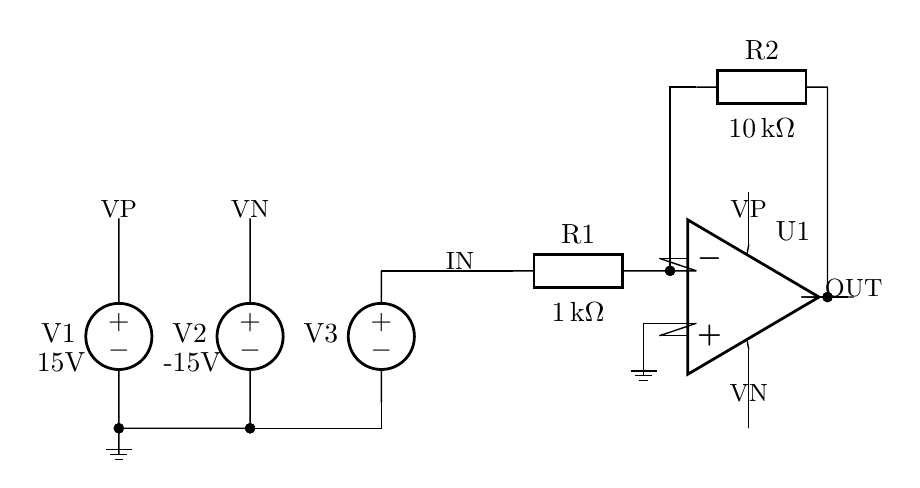
\begin{tikzpicture}[circuit ee IEC, scale=0.6666666667,line width=.5pt]% default: 0.4
            %\tikzstyle{every node}=[font=\small];%
            %\node [draw] at (0.0,0.0) {\pgfkeysvalueof{/tikz/circuitikz/tripoles/op amp/font}};
        \draw [/lt2ti/Net](9.0,1.0)to[*short,-, color=netcolor] (9.0,1.0);% wire w3_w10 start
        \draw [/lt2ti/Net](8.5,-2.5)to[*short,-*, color=netcolor] (8.5,-2.5);% wire w3_w10 end
        \draw [/lt2ti/Net](9.0,1.0) --  (8.5,1.0) -- (8.5,-2.5); % wire w3_w10 polyline 
        \draw [/lt2ti/Net](10.0,-2.0)to[*short,-, color=netcolor] (10.0,-2.0);% wire w4_w5 start
        \draw [/lt2ti/Net](10.0,-1.0)to[*short,-, color=netcolor] (10.0,-1.0);% wire w4_w5 end
        \draw [/lt2ti/Net](10.0,-2.0) --  (10.0,-1.5) -- (10.0,-1.0); % wire w4_w5 polyline 
        \draw [/lt2ti/Net](-2.0,-2.5)to[*short,-, color=netcolor] (-2.0,-1.5);% wire w6
        \draw [/lt2ti/Net](0.5,-2.5)to[*short,-, color=netcolor] (0.5,-1.5);% wire w7
        \draw [/lt2ti/Net](5.5,-2.5)to[*short,-, color=netcolor] (5.5,-2.5);% wire w8_w9 start
        \draw [/lt2ti/Net](3.0,-2.5)to[*short,-, color=netcolor] (3.0,-2.5);% wire w8_w9 end
        \draw [/lt2ti/Net](5.5,-2.5) --  (4.5,-2.5) -- (3.0,-2.5); % wire w8_w9 polyline 
        \draw [/lt2ti/Net](8.5,-2.5)to[*short,*-, color=netcolor] (8.0,-2.5);% wire w11
        \draw [/lt2ti/Net](9.0,-2.5)to[*short,-*, color=netcolor] (8.5,-2.5);% wire w12
        \draw [/lt2ti/Net](11.5,-3.0)to[*short,*-, color=netcolor] (11.5,1.0);% wire w13
        \draw [/lt2ti/Net](11.5,-3.0)to[*short,*-, color=netcolor] (11.0,-3.0);% wire w14
        \draw [/lt2ti/Net](12.0,-3.0)to[*short,-*, color=netcolor] (11.5,-3.0);% wire w15
        \draw [/lt2ti/Net](9.0,-3.5)to[*short,-, color=netcolor] (9.0,-3.5);% wire w16_w17 start
        \draw [/lt2ti/Net](8.0,-4.5)to[*short,-, color=netcolor] (8.0,-4.5);% wire w16_w17 end
        \draw [/lt2ti/Net](9.0,-3.5) --  (8.0,-3.5) -- (8.0,-4.5); % wire w16_w17 polyline 
        \draw [/lt2ti/Net](-2.0,-5.5)to[*short,*-, color=netcolor] (-2.0,-5.0);% wire w19
        \draw [/lt2ti/Net](0.5,-5.5)to[*short,*-, color=netcolor] (0.5,-5.0);% wire w20
        \draw [/lt2ti/Net](0.5,-5.5)to[*short,*-*, color=netcolor] (-2.0,-5.5);% wire w21
        \draw [/lt2ti/Net](3.0,-5.0)to[*short,-, color=netcolor] (3.0,-5.0);% wire w22_w23 start
        \draw [/lt2ti/Net](0.5,-5.5)to[*short,-*, color=netcolor] (0.5,-5.5);% wire w22_w23 end
        \draw [/lt2ti/Net](3.0,-5.0) --  (3.0,-5.5) -- (0.5,-5.5); % wire w22_w23 polyline 
        \draw [/lt2ti/Net](10.0,-5.5)to[*short,-, color=netcolor] (10.0,-5.5);% wire w18_w24 start
        \draw [/lt2ti/Net](10.0,-4.0)to[*short,-, color=netcolor] (10.0,-4.0);% wire w18_w24 end
        \draw [/lt2ti/Net](10.0,-5.5) --  (10.0,-5.0) -- (10.0,-4.0); % wire w18_w24 polyline 
        \draw [/lt2ti/Net](-2.0,-6.0)to[*short,-*, color=netcolor] (-2.0,-5.5);% wire w25
         \draw (8.0, -4.5) node[ground, xscale=1, yscale=1, rotate=270, ] (undefined) {};%  (undefined)++(0.0,0.0) node {undefined }; % component "circuiTikz\gnd" "undefined" 
         \draw (-2.0, -6.0) node[ground, xscale=1, yscale=1, rotate=270, ] (undefined) {};%  (undefined)++(0.0,0.0) node {undefined }; % component "circuiTikz\gnd" "undefined" 
         \draw (10.08863, -3.0) node[op amp, xscale=1, rotate=0, ] (U1) {}  (U1)++(1*0.75,  1*1.25) node {U1 }; % component "OpAmps/ADA4817" "U1" 
         \draw (10.0,-2.0) to [*short, -] (U1.up);   \draw (10.0,-4.0) to [*short, -] (U1.down); % supply % component "OpAmps/ADA4817" "U1" 
         \draw (9.0,-3.5) to [*short, -] (U1.+);   \draw (9.0,-2.5) to [*short, -] (U1.-); \draw (11.0,-3.0) to [*short, -] (U1.out); % in/out % component "OpAmps/ADA4817" "U1" 
          \draw (-2.0, -2.5) to[*V, l_=V1, ,, -, ] (-2.0,-5.0){}; % component "voltage" "V1" 
          \draw (-3.1, -4.8) node[label=15V] {};
          \draw (0.5, -2.5) to[*V, l_=V2, ,, -, ] (0.5,-5.0){}; % component "voltage" "V2" 
          \draw (-0.6, -4.8) node[label=-15V] {};
          \draw (3.0, -2.5) to[*V, l_=V3, a^=,, -, ] (3.0,-5.0){}; % component "voltage" "V3" 
          \draw (8.0, -2.5) to[*resistor, a_=R1, l^=\SI{1}{\kilo\ohm}, -, ] (5.5,-2.5){}; %\node [] at (8.5,-2.0) {x}; % component "res" "R1" 
          \draw (11.5, 1.0) to[*resistor, a_=R2, l^=\SI{10}{\kilo\ohm}, -, ] (9.0,1.0){}; %\node [] at (12.0,1.5) {x}; % component "res" "R2" 
          \node (OUT) [] at (12.0,-3.0) {};% label mark % label "" "OUT" lbl28 
          \node (OUTtxt) [ netlabelcolor, above= -0.24cm of OUT] {{\pgfkeysvalueof{/lt2ti/netlabel/font}OUT}}; % label "" "OUT" lbl28 
          \node (VP) [] at (10.0,-1.5) {};% label mark % label "" "VP" lbl30 
          \node (VPtxt) [ netlabelcolor, above= -0.24cm of VP] {{\pgfkeysvalueof{/lt2ti/netlabel/font}VP}}; % label "" "VP" lbl30 
          \node (VP) [] at (-2.0,-1.5) {};% label mark % label "" "VP" lbl31 
          \node (VPtxt) [ netlabelcolor, above= -0.24cm of VP] {{\pgfkeysvalueof{/lt2ti/netlabel/font}VP}}; % label "" "VP" lbl31 
          \node (VN) [] at (0.5,-1.5) {};% label mark % label "" "VN" lbl32 
          \node (VNtxt) [ netlabelcolor, above= -0.24cm of VN] {{\pgfkeysvalueof{/lt2ti/netlabel/font}VN}}; % label "" "VN" lbl32 
          \node (VN) [] at (10.0,-5.0) {};% label mark % label "" "VN" lbl33 
          \node (VNtxt) [ netlabelcolor, above= -0.24cm of VN] {{\pgfkeysvalueof{/lt2ti/netlabel/font}VN}}; % label "" "VN" lbl33 
          \node (IN) [] at (4.5,-2.5) {};% label mark % label "" "IN" lbl34 
          \node (INtxt) [ netlabelcolor, above= -0.24cm of IN] {{\pgfkeysvalueof{/lt2ti/netlabel/font}IN}}; % label "" "IN" lbl34 
        
            \end{tikzpicture}
        \caption{反転増幅回路(20dB) 回路図}
    \end{center}
\end{figure}

この周波数特性をシュミレーションした結果、以下のような結果が得られた。

\begin{figure}[H]
    \begin{center}
        \includegraphics[width=11cm]{graphing/figures/反転/20dB&40dB(理論曲線あり).png}
        \caption{反転増幅回路 周波数特性}
    \end{center}
\end{figure}

ゲインが3dB落ちたところ(37dBと17dB)に線を引き、遮断周波数をグラフから読み取ると、40dB, 20dBの場合それぞれについて50000Hz, 470000Hzとなっていることがわかる。ここで、色のついている線は理論曲線である。ただし、理論曲線の計算においては上記のように計測した遮断周波数を用いた。\\

また、カットオフ周波数以降の傾きを最大2乗法で調べた結果、以下のようになった。

\begin{table}[H]
    \begin{center}
        \begin{tabular}{|l|c|c|} \hline
            dB & 範囲 & 傾き \\ \hline
            20 & > $1.2\times 10^{6}$Hz & -19.98 \\ \hline
            40 & > $1.0 \times 10^5$Hz & -19.94 \\ \hline
        \end{tabular}
        \caption{反転増幅回路 傾き}
    \end{center}
\end{table}

周波数特性は以下の式で表されることがわかっている。なお、20dB, 40dBの場合において、それぞれ$A_0$は10, 100である。
$$
A(j\omega) = \frac{A_0}{1+j\frac{\omega}{\omega_p}}
$$
よってゲイン特性は
$$
A(j\omega) = \left|\frac{A_0}{1+j\frac{\omega}{\omega_p}}\right|
$$
と表され、$\omega=\omega_p$とすれば
$$
\left|\frac{A_0}{1+j\frac{\omega}{\omega_p}}\right| = \left|\frac{A_0}{1+j}\right| = \frac{A_0}{\sqrt{2}}
$$
となることがわかる。また、$\omega \gg \omega_p$とすると$1+\frac{\omega}{\omega_p} \fallingdotseq \frac{\omega}{\omega_p}$であるから、
$$
\left|\frac{A_0}{1+j\frac{\omega}{\omega_p}}\right| \fallingdotseq A_0\omega_p\omega^{-1}
$$
と表されることから、dB表記では傾きが-20dB/decとなることがわかる。20dB, 40dBの場合において、どちらも誤差率0\%で理論値と一致していることがわかる。\\~\\

\begin{comment}
\begin{figure}[H]
    \begin{center}
	%\centering%
    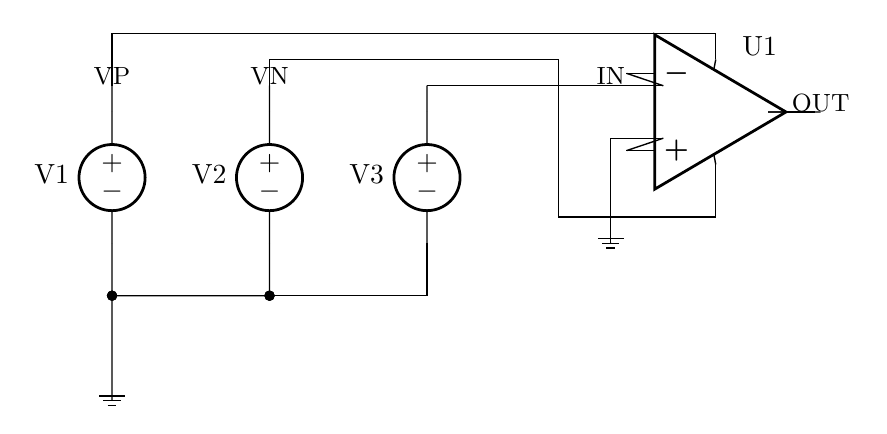
\begin{tikzpicture}[circuit ee IEC, scale=0.666667,line width=.5pt]% default: 0.4
        %\tikzstyle{every node}=[font=\small];%
        %\node [draw] at (0.0,0.0) {\pgfkeysvalueof{/tikz/circuitikz/tripoles/op amp/font}};
    \draw [/lt2ti/Net](-0.5,-7.0)to[*short,-, color=netcolor] (-0.5,-7.0);% wire w4_w3_w6 start
    \draw [/lt2ti/Net](11.0,-6.5)to[*short,-, color=netcolor] (11.0,-6.5);% wire w4_w3_w6 end
    \draw [/lt2ti/Net](-0.5,-7.0) --  (-0.5,-6.0) --  (11.0,-6.0) -- (11.0,-6.5); % wire w4_w3_w6 polyline 
    \draw [/lt2ti/Net](10.0,-7.0)to[*short,-, color=netcolor] (10.0,-7.0);% wire w8_w9 start
    \draw [/lt2ti/Net](5.5,-7.0)to[*short,-, color=netcolor] (5.5,-7.0);% wire w8_w9 end
    \draw [/lt2ti/Net](10.0,-7.0) --  (9.0,-7.0) -- (5.5,-7.0); % wire w8_w9 polyline 
    \draw [/lt2ti/Net](-0.5,-7.5)to[*short,-, color=netcolor] (-0.5,-7.0);% wire w10
    \draw [/lt2ti/Net](2.5,-7.5)to[*short,-, color=netcolor] (2.5,-7.0);% wire w11
    \draw [/lt2ti/Net](5.5,-7.5)to[*short,-, color=netcolor] (5.5,-7.0);% wire w12
    \draw [/lt2ti/Net](13.0,-7.5)to[*short,-, color=netcolor] (12.0,-7.5);% wire w13
    \draw [/lt2ti/Net](10.0,-8.0)to[*short,-, color=netcolor] (10.0,-8.0);% wire w14_w18 start
    \draw [/lt2ti/Net](9.0,-10.0)to[*short,-, color=netcolor] (9.0,-10.0);% wire w14_w18 end
    \draw [/lt2ti/Net](10.0,-8.0) --  (9.0,-8.0) -- (9.0,-10.0); % wire w14_w18 polyline 
    \draw [/lt2ti/Net](11.0,-8.5)to[*short,-, color=netcolor] (11.0,-8.5);% wire w16_w17_w7_w5_w15 start
    \draw [/lt2ti/Net](2.5,-7.0)to[*short,-, color=netcolor] (2.5,-7.0);% wire w16_w17_w7_w5_w15 end
    \draw [/lt2ti/Net](11.0,-8.5) --  (11.0,-9.5) --  (8.0,-9.5) --  (8.0,-6.5) --  (2.5,-6.5) -- (2.5,-7.0); % wire w16_w17_w7_w5_w15 polyline 
    \draw [/lt2ti/Net](-0.5,-11.0)to[*short,*-, color=netcolor] (-0.5,-10.0);% wire w19
    \draw [/lt2ti/Net](2.5,-11.0)to[*short,*-, color=netcolor] (2.5,-10.0);% wire w20
    \draw [/lt2ti/Net](2.5,-11.0)to[*short,*-*, color=netcolor] (-0.5,-11.0);% wire w21
    \draw [/lt2ti/Net](5.5,-10.0)to[*short,-, color=netcolor] (5.5,-10.0);% wire w22_w23 start
    \draw [/lt2ti/Net](2.5,-11.0)to[*short,-*, color=netcolor] (2.5,-11.0);% wire w22_w23 end
    \draw [/lt2ti/Net](5.5,-10.0) --  (5.5,-11.0) -- (2.5,-11.0); % wire w22_w23 polyline 
    \draw [/lt2ti/Net](-0.5,-13.0)to[*short,-*, color=netcolor] (-0.5,-11.0);% wire w24
     \draw (-0.5, -13.0) node[ground, xscale=1, yscale=1, rotate=270, ] (undefined) {};%  (undefined)++(0.0,0.0) node {undefined }; % component "circuiTikz\gnd" "undefined" 
     \draw (9.0, -10.0) node[ground, xscale=1, yscale=1, rotate=270, ] (undefined) {};%  (undefined)++(0.0,0.0) node {undefined }; % component "circuiTikz\gnd" "undefined" 
     \draw (11.08863, -7.5) node[op amp, xscale=1, rotate=0, ] (U1) {}  (U1)++(1*0.75,  1*1.25) node {U1 }; % component "OpAmps/ADA4817" "U1" 
     \draw (11.0,-6.5) to [*short, -] (U1.up);   \draw (11.0,-8.5) to [*short, -] (U1.down); % supply % component "OpAmps/ADA4817" "U1" 
     \draw (10.0,-8.0) to [*short, -] (U1.+);   \draw (10.0,-7.0) to [*short, -] (U1.-); \draw (12.0,-7.5) to [*short, -] (U1.out); % in/out % component "OpAmps/ADA4817" "U1" 
      \draw (-0.5, -7.5) to[*V, l_=V1,, -, ] (-0.5,-10.0){}; % component "voltage" "V1" 
      \draw (2.5, -7.5) to[*V, l_=V2,, -, ] (2.5,-10.0){}; % component "voltage" "V2" 
      \draw (5.5, -7.5) to[*V, l_=V3,, -, ] (5.5,-10.0){}; % component "voltage" "V3" 
      \node (OUT) [] at (13.0,-7.5) {};% label mark % label "" "OUT" lbl27 
      \node (OUTtxt) [ netlabelcolor, above= -0.24cm of OUT] {{\pgfkeysvalueof{/lt2ti/netlabel/font}OUT}}; % label "" "OUT" lbl27 
      \node (VP) [] at (-0.5,-7.0) {};% label mark % label "" "VP" lbl29 
      \node (VPtxt) [ netlabelcolor, above= -0.24cm of VP] {{\pgfkeysvalueof{/lt2ti/netlabel/font}VP}}; % label "" "VP" lbl29 
      \node (VN) [] at (2.5,-7.0) {};% label mark % label "" "VN" lbl30 
      \node (VNtxt) [ netlabelcolor, above= -0.24cm of VN] {{\pgfkeysvalueof{/lt2ti/netlabel/font}VN}}; % label "" "VN" lbl30 
      \node (IN) [] at (9.0,-7.0) {};% label mark % label "" "IN" lbl31 
      \node (INtxt) [ netlabelcolor, above= -0.24cm of IN] {{\pgfkeysvalueof{/lt2ti/netlabel/font}IN}}; % label "" "IN" lbl31 
    
        \end{tikzpicture}
        \caption{反転増幅回路 回路図}
    \end{center}
\end{figure}

\end{comment}

非反転増幅回路については、$増幅率 = \frac{V_out}{V_in} = \frac{R1+R2}{R2}$が20dB, 40dBとなるようにすれば良い。回路図は以下のようになる。

\begin{figure}[H]
    \begin{center}
        %\centering%
		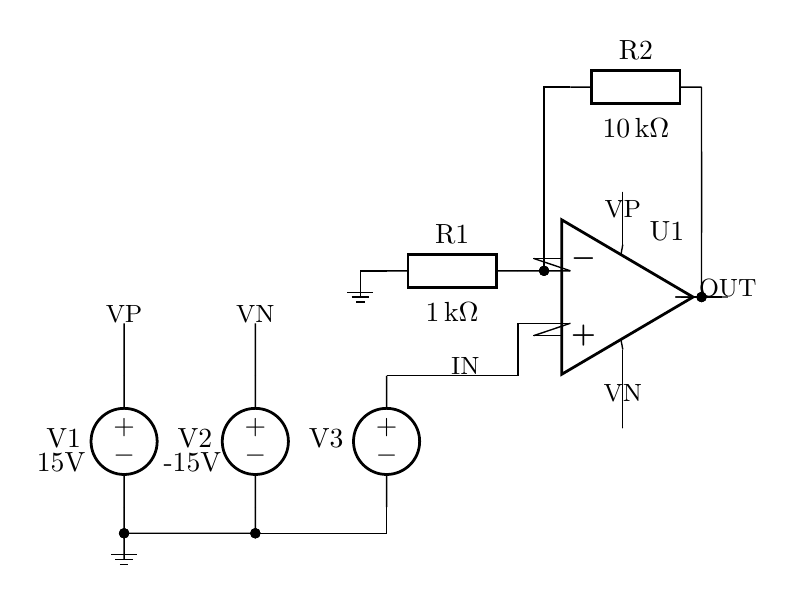
\begin{tikzpicture}[circuit ee IEC, scale=0.6666666667,line width=.5pt]% default: 0.4
            %\tikzstyle{every node}=[font=\small];%
            %\node [draw] at (0.0,0.0) {\pgfkeysvalueof{/tikz/circuitikz/tripoles/op amp/font}};
        \draw [/lt2ti/Net](9.0,1.0)to[*short,-, color=netcolor] (9.0,1.0);% wire w3_w7 start
        \draw [/lt2ti/Net](8.5,-2.5)to[*short,-*, color=netcolor] (8.5,-2.5);% wire w3_w7 end
        \draw [/lt2ti/Net](9.0,1.0) --  (8.5,1.0) -- (8.5,-2.5); % wire w3_w7 polyline 
        \draw [/lt2ti/Net](10.0,-2.0)to[*short,-, color=netcolor] (10.0,-2.0);% wire w4_w5 start
        \draw [/lt2ti/Net](10.0,-1.0)to[*short,-, color=netcolor] (10.0,-1.0);% wire w4_w5 end
        \draw [/lt2ti/Net](10.0,-2.0) --  (10.0,-1.5) -- (10.0,-1.0); % wire w4_w5 polyline 
        \draw [/lt2ti/Net](5.5,-2.5)to[*short,-, color=netcolor] (5.5,-2.5);% wire w6_w10 start
        \draw [/lt2ti/Net](5.0,-3.0)to[*short,-, color=netcolor] (5.0,-3.0);% wire w6_w10 end
        \draw [/lt2ti/Net](5.5,-2.5) --  (5.0,-2.5) -- (5.0,-3.0); % wire w6_w10 polyline 
        \draw [/lt2ti/Net](8.5,-2.5)to[*short,*-, color=netcolor] (8.0,-2.5);% wire w8
        \draw [/lt2ti/Net](9.0,-2.5)to[*short,-*, color=netcolor] (8.5,-2.5);% wire w9
        \draw [/lt2ti/Net](11.5,-3.0)to[*short,*-, color=netcolor] (11.5,1.0);% wire w11
        \draw [/lt2ti/Net](11.5,-3.0)to[*short,*-, color=netcolor] (11.0,-3.0);% wire w12
        \draw [/lt2ti/Net](12.0,-3.0)to[*short,-*, color=netcolor] (11.5,-3.0);% wire w13
        \draw [/lt2ti/Net](9.0,-3.5)to[*short,-, color=netcolor] (9.0,-3.5);% wire w14_w18_w17_w19 start
        \draw [/lt2ti/Net](5.5,-4.5)to[*short,-, color=netcolor] (5.5,-4.5);% wire w14_w18_w17_w19 end
        \draw [/lt2ti/Net](9.0,-3.5) --  (8.0,-3.5) --  (8.0,-4.5) --  (7.0,-4.5) -- (5.5,-4.5); % wire w14_w18_w17_w19 polyline 
        \draw [/lt2ti/Net](0.5,-4.5)to[*short,-, color=netcolor] (0.5,-3.5);% wire w15
        \draw [/lt2ti/Net](3.0,-4.5)to[*short,-, color=netcolor] (3.0,-3.5);% wire w16
        \draw [/lt2ti/Net](10.0,-5.5)to[*short,-, color=netcolor] (10.0,-5.5);% wire w20_w21 start
        \draw [/lt2ti/Net](10.0,-4.0)to[*short,-, color=netcolor] (10.0,-4.0);% wire w20_w21 end
        \draw [/lt2ti/Net](10.0,-5.5) --  (10.0,-5.0) -- (10.0,-4.0); % wire w20_w21 polyline 
        \draw [/lt2ti/Net](0.5,-7.5)to[*short,*-, color=netcolor] (0.5,-7.0);% wire w22
        \draw [/lt2ti/Net](3.0,-7.5)to[*short,*-, color=netcolor] (3.0,-7.0);% wire w23
        \draw [/lt2ti/Net](3.0,-7.5)to[*short,*-*, color=netcolor] (0.5,-7.5);% wire w24
        \draw [/lt2ti/Net](5.5,-7.0)to[*short,-, color=netcolor] (5.5,-7.0);% wire w25_w26 start
        \draw [/lt2ti/Net](3.0,-7.5)to[*short,-*, color=netcolor] (3.0,-7.5);% wire w25_w26 end
        \draw [/lt2ti/Net](5.5,-7.0) --  (5.5,-7.5) -- (3.0,-7.5); % wire w25_w26 polyline 
        \draw [/lt2ti/Net](0.5,-8.0)to[*short,-*, color=netcolor] (0.5,-7.5);% wire w27
         \draw (5.0, -3.0) node[ground, xscale=1, yscale=1, rotate=270, ] (undefined) {};%  (undefined)++(0.0,0.0) node {undefined }; % component "circuiTikz\gnd" "undefined" 
         \draw (0.5, -8.0) node[ground, xscale=1, yscale=1, rotate=270, ] (undefined) {};%  (undefined)++(0.0,0.0) node {undefined }; % component "circuiTikz\gnd" "undefined" 
         \draw (10.08863, -3.0) node[op amp, xscale=1, rotate=0, ] (U1) {}  (U1)++(1*0.75,  1*1.25) node {U1 }; % component "OpAmps/ADA4817" "U1" 
         \draw (10.0,-2.0) to [*short, -] (U1.up);   \draw (10.0,-4.0) to [*short, -] (U1.down); % supply % component "OpAmps/ADA4817" "U1" 
         \draw (9.0,-3.5) to [*short, -] (U1.+);   \draw (9.0,-2.5) to [*short, -] (U1.-); \draw (11.0,-3.0) to [*short, -] (U1.out); % in/out % component "OpAmps/ADA4817" "U1" 
          \draw (0.5, -4.5) to[*V, l_=V1,,, -, ] (0.5,-7.0){}; % component "voltage" "V1" 
          \draw (-0.7, -6.7) node[label=15V]{};
          \draw (3.0, -4.5) to[*V, l_=V2,,, -, ] (3.0,-7.0){}; % component "voltage" "V2" 
          \draw (1.8, -6.7) node[label=-15V] {};
          \draw (5.5, -4.5) to[*V, l_=V3, a^=,, -, ] (5.5,-7.0){}; % component "voltage" "V3" 
          \draw (8.0, -2.5) to[*resistor, a_=R1, l^=\SI{1}{\kilo\ohm}, -, ] (5.5,-2.5){}; %\node [] at (8.5,-2.0) {x}; % component "res" "R1" 
          \draw (11.5, 1.0) to[*resistor, a_=R2, l^=\SI{10}{\kilo\ohm}, -, ] (9.0,1.0){}; %\node [] at (12.0,1.5) {x}; % component "res" "R2" 
          \node (OUT) [] at (12.0,-3.0) {};% label mark % label "" "OUT" lbl30 
          \node (OUTtxt) [ netlabelcolor, above= -0.24cm of OUT] {{\pgfkeysvalueof{/lt2ti/netlabel/font}OUT}}; % label "" "OUT" lbl30 
          \node (VP) [] at (10.0,-1.5) {};% label mark % label "" "VP" lbl32 
          \node (VPtxt) [ netlabelcolor, above= -0.24cm of VP] {{\pgfkeysvalueof{/lt2ti/netlabel/font}VP}}; % label "" "VP" lbl32 
          \node (VP) [] at (0.5,-3.5) {};% label mark % label "" "VP" lbl33 
          \node (VPtxt) [ netlabelcolor, above= -0.24cm of VP] {{\pgfkeysvalueof{/lt2ti/netlabel/font}VP}}; % label "" "VP" lbl33 
          \node (VN) [] at (3.0,-3.5) {};% label mark % label "" "VN" lbl34 
          \node (VNtxt) [ netlabelcolor, above= -0.24cm of VN] {{\pgfkeysvalueof{/lt2ti/netlabel/font}VN}}; % label "" "VN" lbl34 
          \node (VN) [] at (10.0,-5.0) {};% label mark % label "" "VN" lbl35 
          \node (VNtxt) [ netlabelcolor, above= -0.24cm of VN] {{\pgfkeysvalueof{/lt2ti/netlabel/font}VN}}; % label "" "VN" lbl35 
          \node (IN) [] at (7.0,-4.5) {};% label mark % label "" "IN" lbl36 
          \node (INtxt) [ netlabelcolor, above= -0.24cm of IN] {{\pgfkeysvalueof{/lt2ti/netlabel/font}IN}}; % label "" "IN" lbl36 
        
            \end{tikzpicture}

        \caption{非反転増幅回路}
    \end{center}
\end{figure}

この回路のシミュレーションした結果、以下のような周波数特性が得られた。

\begin{figure}[H]
    \begin{center}
        \includegraphics[width=11cm]{graphing/figures/非反転/20dB&40dB(理論曲線あり).png}
        \caption{非反転増幅回路 周波数特性}
    \end{center}
\end{figure}

ゲインが3dB落ちたところ(37dBと17dB)に線を引き、遮断周波数をグラフから夜mいm取ると、40dB, 20dbの場合それぞれについて50000Hz, 470000Hzとなっていることがわかる。反転増幅回路の周波数特性のグラフと同様に、色のついてる線は理論曲線である。
\\
カットオフ周波数以降の傾きを最大2乗法で調べた結果、以下のようになった。

\begin{table}[H]
    \begin{center}
        \begin{tabular}{|l|c|c|} \hline
            dB & 範囲 & 傾き \\ \hline
            20 & > $1.0\times 10^{6}$Hz & -19.96 \\ \hline
            40 & > $1.0 \times 10^5$Hz & -19.95 \\ \hline
        \end{tabular}
        \caption{非反転増幅回路 傾き}
    \end{center}
\end{table}

周波数特性については同様の式で表され、dB表記では傾きが-20dB/decとなることがわかり、20dB, 40dBの場合それぞれについてどちらも誤差率0\%で理論値と一致していることがわかる。
\\~\\
(2)今回の微分回路の閉ループ利得は極箇所式A2.41から
$$
\frac{V_o(s)}{V_r(s)} = \frac{sC_rR_f}{(sC_rR_r + 1)(sC_fR_f + 1)}
$$
と与えられる。それぞれの波形は以下のような形となった。
\begin{figure}[H]
    \begin{center}
        \includegraphics[width=11cm]{graphing/figures/微分/with_rrcf.png}
        \caption{微分増幅器 波形}
    \end{center}
\end{figure}

微分回路は$f < f_r$において微分特性を示し、$f_r < f < f_f$において反転増幅を示し、$f_f < f$において積分特性を示す。50Hz, 5000Hz, $5\times10^8Hz$の電圧を流した際の周波数応答の結果が以下である。
\begin{figure}[H]
    \begin{center}
        \includegraphics[width=11cm]{graphing/figures/ステップ/微分.png}
        \caption{f = 50Hzの微分回路の周波数特性}
    \end{center}
\end{figure}

\begin{figure}[H]
    \begin{center}
        \includegraphics[width=11cm]{graphing/figures/ステップ/反転.png}
        \caption{f = 5000Hzの微分回路の周波数特性}
    \end{center}
\end{figure}

\begin{figure}[H]
    \begin{center}
        \includegraphics[width=11cm]{graphing/figures/ステップ/積分.png}
        \caption{f = $5.0\times 10^8$Hzの微分回路の周波数特性}
    \end{center}
\end{figure}

\subsection*{8.2}
(1)ウィーンブリッジは以下のような回路である。

\begin{figure}[H]
    \begin{center}
        %\centering%
        \begin{adjustbox}{scale=0.7}
            \begin{tikzpicture}[circuit ee IEC, scale=0.66666667,line width=.5pt]% default: 0.4
            %\tikzstyle{every node}=[font=\small];%
            %\node [draw] at (0.0,0.0) {\pgfkeysvalueof{/tikz/circuitikz/tripoles/op amp/font}};
        \draw [/lt2ti/Net](12.5,-9.0)to[*short,-, color=netcolor] (12.5,-9.0);% wire w3_w8 start
        \draw [/lt2ti/Net](11.5,-13.0)to[*short,-*, color=netcolor] (11.5,-13.0);% wire w3_w8 end
        \draw [/lt2ti/Net](12.5,-9.0) --  (11.5,-9.0) -- (11.5,-13.0); % wire w3_w8 polyline 
        \draw [/lt2ti/Net](13.5,-11.5)to[*short,-, color=netcolor] (13.5,-11.0);% wire w5
        \draw [/lt2ti/Net](13.5,-12.5)to[*short,-, color=netcolor] (13.5,-11.5);% wire w6
        \draw [/lt2ti/Net](8.0,-13.0)to[*short,-, color=netcolor] (8.0,-13.0);% wire w7_w16 start
        \draw [/lt2ti/Net](6.5,-14.5)to[*short,-, color=netcolor] (6.5,-14.5);% wire w7_w16 end
        \draw [/lt2ti/Net](8.0,-13.0) --  (6.5,-13.0) -- (6.5,-14.5); % wire w7_w16 polyline 
        \draw [/lt2ti/Net](11.5,-13.0)to[*short,*-, color=netcolor] (10.5,-13.0);% wire w9
        \draw [/lt2ti/Net](12.5,-13.0)to[*short,-*, color=netcolor] (11.5,-13.0);% wire w10
        \draw [/lt2ti/Net](17.0,-13.5)to[*short,*-, color=netcolor] (14.5,-13.5);% wire w12
        \draw [/lt2ti/Net](17.0,-13.5)to[*short,*-, color=netcolor] (17.0,-13.5);% wire w4_w11 start
        \draw [/lt2ti/Net](15.0,-9.0)to[*short,-, color=netcolor] (15.0,-9.0);% wire w4_w11 end
        \draw [/lt2ti/Net](17.0,-13.5) --  (17.0,-9.0) -- (15.0,-9.0); % wire w4_w11 polyline 
        \draw [/lt2ti/Net](23.0,-13.5)to[*short,*-*, color=netcolor] (17.0,-13.5);% wire w13
        \draw [/lt2ti/Net](23.0,-13.5)to[*short,*-, color=netcolor] (23.0,-13.5);% wire w22_w23 start
        \draw [/lt2ti/Net](22.5,-15.5)to[*short,-, color=netcolor] (22.5,-15.5);% wire w22_w23 end
        \draw [/lt2ti/Net](23.0,-13.5) --  (23.0,-15.5) -- (22.5,-15.5); % wire w22_w23 polyline 
        \draw [/lt2ti/Net](24.5,-13.5)to[*short,-*, color=netcolor] (23.0,-13.5);% wire w14
        \draw [/lt2ti/Net](13.5,-15.5)to[*short,-, color=netcolor] (13.5,-14.5);% wire w19
        \draw [/lt2ti/Net](17.5,-15.5)to[*short,*-, color=netcolor] (17.5,-15.5);% wire w20_w26 start
        \draw [/lt2ti/Net](15.5,-16.0)to[*short,-, color=netcolor] (15.5,-16.0);% wire w20_w26 end
        \draw [/lt2ti/Net](17.5,-15.5) --  (15.5,-15.5) -- (15.5,-16.0); % wire w20_w26 polyline 
        \draw [/lt2ti/Net](18.0,-15.5)to[*short,-*, color=netcolor] (17.5,-15.5);% wire w21
        \draw [/lt2ti/Net](1.0,-16.0)to[*short,-, color=netcolor] (1.0,-16.0);% wire w17_w24 start
        \draw [/lt2ti/Net](1.0,-13.0)to[*short,-, color=netcolor] (1.0,-13.0);% wire w17_w24 end
        \draw [/lt2ti/Net](1.0,-16.0) --  (1.0,-15.0) -- (1.0,-13.0); % wire w17_w24 polyline 
        \draw [/lt2ti/Net](4.0,-16.0)to[*short,-, color=netcolor] (4.0,-16.0);% wire w18_w25 start
        \draw [/lt2ti/Net](4.0,-13.0)to[*short,-, color=netcolor] (4.0,-13.0);% wire w18_w25 end
        \draw [/lt2ti/Net](4.0,-16.0) --  (4.0,-15.0) -- (4.0,-13.0); % wire w18_w25 polyline 
        \draw [/lt2ti/Net](17.5,-17.5)to[*short,-*, color=netcolor] (17.5,-15.5);% wire w27
        \draw [/lt2ti/Net](15.5,-19.0)to[*short,*-, color=netcolor] (15.5,-18.5);% wire w29
        \draw [/lt2ti/Net](15.5,-19.0)to[*short,*-, color=netcolor] (15.5,-19.0);% wire w30_w15_w28 start
        \draw [/lt2ti/Net](12.5,-14.0)to[*short,-, color=netcolor] (12.5,-14.0);% wire w30_w15_w28 end
        \draw [/lt2ti/Net](15.5,-19.0) --  (11.5,-19.0) --  (11.5,-14.0) -- (12.5,-14.0); % wire w30_w15_w28 polyline 
        \draw [/lt2ti/Net](1.0,-20.5)to[*short,*-, color=netcolor] (1.0,-18.5);% wire w31
        \draw [/lt2ti/Net](4.0,-18.5)to[*short,-, color=netcolor] (4.0,-18.5);% wire w32_w33 start
        \draw [/lt2ti/Net](1.0,-20.5)to[*short,-*, color=netcolor] (1.0,-20.5);% wire w32_w33 end
        \draw [/lt2ti/Net](4.0,-18.5) --  (4.0,-20.5) -- (1.0,-20.5); % wire w32_w33 polyline 
        \draw [/lt2ti/Net](1.0,-22.0)to[*short,-*, color=netcolor] (1.0,-20.5);% wire w34
        \draw [/lt2ti/Net](15.5,-22.0)to[*short,*-, color=netcolor] (15.5,-21.5);% wire w35
        \draw [/lt2ti/Net](17.5,-19.5)to[*short,-, color=netcolor] (17.5,-19.5);% wire w36_w37 start
        \draw [/lt2ti/Net](15.5,-22.0)to[*short,-*, color=netcolor] (15.5,-22.0);% wire w36_w37 end
        \draw [/lt2ti/Net](17.5,-19.5) --  (17.5,-22.0) -- (15.5,-22.0); % wire w36_w37 polyline 
        \draw [/lt2ti/Net](15.5,-22.5)to[*short,-*, color=netcolor] (15.5,-22.0);% wire w38
         \draw (6.5, -14.5) node[ground, xscale=1, yscale=1, rotate=270, ] (undefined) {};%  (undefined)++(0.0,0.0) node {undefined }; % component "circuiTikz\gnd" "undefined" 
         \draw (1.0, -22.0) node[ground, xscale=1, yscale=1, rotate=270, ] (undefined) {};%  (undefined)++(0.0,0.0) node {undefined }; % component "circuiTikz\gnd" "undefined" 
         \draw (15.5, -22.5) node[ground, xscale=1, yscale=1, rotate=270, ] (undefined) {};%  (undefined)++(0.0,0.0) node {undefined }; % component "circuiTikz\gnd" "undefined" 
         \draw (13.58863, -13.5) node[op amp, xscale=1, rotate=0, ] (U1) {}  (U1)++(1*0.75,  1*1.25) node {U1 }; % component "OpAmps/ADA4817" "U1" 
         \draw (13.5,-12.5) to [*short, -] (U1.up);   \draw (13.5,-14.5) to [*short, -] (U1.down); % supply % component "OpAmps/ADA4817" "U1" 
         \draw (12.5,-14.0) to [*short, -] (U1.+);   \draw (12.5,-13.0) to [*short, -] (U1.-); \draw (14.5,-13.5) to [*short, -] (U1.out); % in/out % component "OpAmps/ADA4817" "U1" 
          \draw (1.0, -16.0) to[*V, l_=V1,, -, ] (1.0,-18.5){}; % component "voltage" "V1" 
          \draw (-0.2, -18.3) node[label=15V] {};
          \draw (4.0, -16.0) to[*V, l_=V2,, -, ] (4.0,-18.5){}; % component "voltage" "V2" 
          \draw (2.9, -18.3) node[label=-15V] {};
          \draw (10.5, -13.0) to[*resistor, a_=R1, l^=$\SI{1}{\kohm}$, -, ] (8.0,-13.0){}; %\node [] at (11.0,-12.5) {x}; % component "res" "R1" 
          \draw (15.0, -9.0) to[*resistor, a_=R2, l^=$\SI{5}{\kohm}$, -, ] (12.5,-9.0){}; %\node [] at (15.5,-8.5) {x}; % component "res" "R2" 
          \draw (22.5, -15.5) to[*resistor, a_=R3, l^=$\SI{10}{\kohm}$, -, ] (20.0,-15.5){}; %\node [] at (23.0,-15.0) {x}; % component "res" "10K" 
          \draw (20.0, -15.5) to[*capacitor, a_=C1, l^=$\SI{16.7}{\nano\farad}$, -, ] (18.0,-15.5){}; % component "cap" "C1" 
          %\node [] at (20.0,-15.0) {x}; % component "cap" "C1" 
          \draw (15.5, -16.0) to[*resistor, l^=R4, a_=, -, ] (15.5,-18.5){}; %\node [] at (15.0,-15.5) {x}; % component "res" "R4" 
          \draw (15.5, -19.0) to[*resistor, l^=R5, a_=, *-, ] (15.5,-21.5){}; %\node [] at (15.0,-18.5) {x}; % component "res" "R5" 
          \draw (17.5, -17.5) to[*capacitor, l^=C2, , -, ] (17.5,-19.5){}; % component "cap" "C2" 
          \draw (19, -19.5) node[label=$\SI{16.7}{\nano\farad}$] {} ;
          %\node [] at (17.0,-17.5) {x}; % component "cap" "C2" 
          \node (VP) [] at (1.0,-15.0) {};% label mark % label "" "VP" lbl40 
          \node (VPtxt) [ netlabelcolor, above= -0.24cm of VP] {{\pgfkeysvalueof{/lt2ti/netlabel/font}VP}}; % label "" "VP" lbl40 
          \node (VP) [] at (13.5,-11.5) {};% label mark % label "" "VP" lbl41 
          \node (VPtxt) [ netlabelcolor, above= -0.24cm of VP] {{\pgfkeysvalueof{/lt2ti/netlabel/font}VP}}; % label "" "VP" lbl41 
          \node (VN) [] at (13.5,-15.5) {};% label mark % label "" "VN" lbl42 
          \node (VNtxt) [ netlabelcolor, above= -0.24cm of VN] {{\pgfkeysvalueof{/lt2ti/netlabel/font}VN}}; % label "" "VN" lbl42 
          \node (VN) [] at (4.0,-15.0) {};% label mark % label "" "VN" lbl43 
          \node (VNtxt) [ netlabelcolor, above= -0.24cm of VN] {{\pgfkeysvalueof{/lt2ti/netlabel/font}VN}}; % label "" "VN" lbl43 
          \node (OUT) [] at (24.5,-13.5) {};% label mark % label "" "OUT" lbl45 
          \node (OUTtxt) [ netlabelcolor, above= -0.24cm of OUT] {{\pgfkeysvalueof{/lt2ti/netlabel/font}OUT}}; % label "" "OUT" lbl45 
            \end{tikzpicture}
        \end{adjustbox}
        \caption{ウィーンブリッジ 回路図}
    \end{center}
\end{figure}

この回路をシミューレーションし、周波数特性を得た。

\begin{figure}[H]
    \begin{center}
        \includegraphics[width=11cm]{graphing/figures/ウィーンブリッジ/k=0.3.png}
        \caption{ウィーンブリッジの周波数特性(k=0.3)}
    \end{center}
\end{figure}

\begin{figure}[H]
    \begin{center}
        \includegraphics[width=11cm]{graphing/figures/ウィーンブリッジ/k=0.501.png}
        \caption{ウィーンブリッジの周波数特性(k=0.501)}
    \end{center}
\end{figure}

シミュレーションの結果から、$k = 0.501$のときに発振している。また、ウィーンブリッジの帰還を切断し、開ループ利得の周波数応答を観測した結果が以下である。

\begin{figure}[H]
    \begin{center}
        \includegraphics[width=11cm]{graphing/figures/ウィーンブリッジ/openloop.png}
        \caption{開ループ利得}
    \end{center}
\end{figure}

ここで、グラフは極大値が小さい方から準に、kの値が0.110, 0.210, 0.310, 0.410, 0.510, 0.610, 0.710, 0.810, 0.910である。また、ゲインの極大値がちょうど0となる直前の線を青とした。この線はk=0.510の線である。

ウィーンブリッジの閉ループ利得$A_v$は以下である。
$$
A_v(s) = A\frac{(sCR)^2+3sCR+1}{(sCR)^2+(3-kA)sCR+1} 
$$
Aは非反転増幅回路の増幅率である。R1 = 1, R2 = 5なのでゲインは$\frac{R1+R2}{R1} = 6$である。また、開ループゲインを計測すると、ゲインが15.56dBであったので5.99となった。この回路は$\omega CR = 1$, $k=3/A$で発信するが、$A=5.99$、$\omega CR = 1$、$k=0.5008$、($s=j\omega$)を上の式の分母に代入すると
$$
(sCR)^2 + (3-kA)sCR + 1 = -(\omega CR)^2 + (3-kA)j\omega CR + 1 = 0
$$
となることから、k=5.008でこの回路は発信することがわかる。

(2) 
k=0.8で通した結果が以下である。
\begin{figure}[H]
    \begin{center}
        \includegraphics[width=11cm]{graphing/figures/ウィーンブリッジ/k=0.501.png}
        \caption{ウィーンブリッジの周波数特性(k=0.501)}
    \end{center}
\end{figure}

これを見ると、これはk>0.501であるが発振していることがわかる。この理由を考える。

kの値を0から1へと変化させた際、
$$
(sCR)^2 + (3-kA)sCR + 1 = 0
$$
の解を考える。s=0となるのは解の公式から
$$
s = \frac{-(3-kA)CR \pm \sqrt{((3-kA)CR)^2 - 4(CR)^2}}{2(CR)^2}
$$
のときであるから、この値がkによってどう変化するかを考える。今回用いた値は$C = 16.7nF$, $R = 10000\Omega$, $A=6$であるから、kを0から変化させたときのsの動きを追ったものが以下である。ただし、$\pm$によって2つに分岐している。
\begin{figure}[H]
    \begin{center}
        \includegraphics[width=11cm]{graphing/figures/circle.png}
        \caption{sの軌道}
    \end{center}
\end{figure}
このように、k=0.5を境に右反面にsが入ることがわかる。

\section{参考文献}
『title』\url{<url>} 2021年n月m日アクセス
\end{document}